%scb-term-paper.tex 
\documentclass[12pt]{article}
\usepackage{times}
\usepackage{amsmath,amssymb,latexsym}
\usepackage[round,sort]{natbib}
\usepackage{multirow,array}
\usepackage{fancyhdr}
\usepackage{lastpage}
\usepackage{graphicx}
\usepackage[bottom]{footmisc}
\graphicspath{ {scb-term-paper-images/} }
\usepackage[T1]{fontenc}
\usepackage{mathptmx}
\usepackage{tabu}
\usepackage{textcomp}
\usepackage{stata}
\usepackage{listings}
\usepackage[a4paper,margin=1.0in]{geometry}
\usepackage{multirow}
\usepackage{caption}
\usepackage{setspace}
\usepackage{verbatim}
\usepackage{pdflscape}
\usepackage{longtable}
\usepackage{hyperref}
\hypersetup{
    colorlinks=true,
    linkcolor=blue,
    filecolor=magenta,      
    urlcolor=cyan,
    citecolor=magenta,
}
\lstset{
basicstyle=\ttfamily,
columns=flexible,
breaklines=true
}
\newenvironment{hypothesis}{
  	\itshape
  	\leftskip=\parindent \rightskip=\parindent
  	\noindent\ignorespaces}
	
\setlength\parindent{0pt}
\pagestyle{fancy}
\fancyhf{}
\lhead{Strategy Content (B) Term Paper}
\rfoot{Page \thepage  \ of \pageref{LastPage}}
\rhead{Iyenggar}
\newcommand\question[2]{\vspace{1em}\hrule\vspace{1em}\textbf{#1}{ #2}\vspace{1em}\hrule\vspace{1em}}

\begin{document}
\title{\LARGE Heterogeneity in knowledge spillovers across regions:\\ \Large The effects of endogeneity,  complexity and IPR environment}
\author{Ashwin Iyenggar  (1521001) \\ ashwin.iyenggar15@iimb.ernet.in} 
\large

\maketitle
\thispagestyle{empty}

\begin{abstract}
\large \noindent I line up empirical evidence to demonstrate the heterogeneity in the geographical distribution of knowledge spillovers across various regions. I then explore  three potential mechanisms that may help explain this heterogeneity: endogenous aspects of the regions themselves, complexity of work, and the intellectual property rights environment of the location. While the empirical results are yet inconclusive and incomplete, the current work extends prior work on geographic spillovers of knowledge by  integrating three hitherto alternative explanations.
\end{abstract}
{Keywords:} Knowledge Spillovers, Endogeniety, Complexity, IPR
\doublespacing
\section{Introduction}
There has been a long and illustrious scholarly tradition highlighting the agglomeration characteristics of economic regions, going back at least as far as \cite{Marshall1890}, whose original work was published in 1890. More recently, scholars over the last three decades have demonstrated the paper trail of these knowledge spillovers through the study of patent citations (e.g., \cite{Jaffe1993, Almeida1999}). This tradition of scholarship has further shaped our theoretical understanding of knowledge spillovers through mechanisms such as the effects of inventor mobility (e.g., \cite{Almeida1999}), differential Intellectual Property Rights environments across locations (e.g., \cite{Zhao2006}) and of the role of international geography (e.g., \cite{Singh2007}).  The nature and extent of the geographical distribution of knowledge spillovers observed  in practice is so highly heterogenous across locations, firms and legal environments,  that the understanding of the causal mechanisms leading to knowledge spillovers continues to intrigue the best of scholars. While this is, in no way dismissive of  the enormous theoretical strides so far, the question is assumes greater significance in the environment surrounding the second machine age as some scholars have begun to highlight \citep{Mcafee2014} 
\\\\
Motivated by empirical evidence surrounding the heterogeneity in the nature of knowledge flows across the various regions, I intend to explore the three mechanisms ostensibly influencing knowledge spillovers. Complexity of patents invented as a potential mechanism influencing the extent of local knowledge spillovers. This approach is not to be construed as yet another mechanical departure from the current theory on spillovers. I argue so with the following reasons.  First, from a human capital perspective, it is valuable to understand the impact of MNCs that dominate much of the cutting- and bleeding-edge innovation in emerging markets on the development of the talent pool in the host country. Does a significant group of local inventors develop? Is this affected by the strength of the IPR regime in the host country? Second, a specific flavor of this question is the investigation of the spillover effects of the innovation process in emerging countries, or those known to have weaker IPR regimes. Specifically, do multinational firms that develop patentable technologies in emerging (or weaker IPR) countries create spillover effects in the host country talent pool? Or do the benefits remain localized to within multinational companies (MNCs) and their home country employees?  Finally, the wide disparity in the extent of knowledge spillovers across locations, across firms and across IPR regimes is intriguing to the researcher and calls attention toward a creative response.  a researcher to find the mechanisms that may lie behind such a phenomenon. Patents data allows us to ask these questions and to have them answered as has been in the tradition of \cite{Jaffe1993}.
\\\\
\begin{figure}[h]
\begin{centering}
  \includegraphics[width=\textwidth]{SameRegionDiffAssigneeFlows}
  \caption{Local and External Flows by Region}
  \label{fig:SameRegionDiffAssigneeFlows}
\end{centering}
\end{figure}
The choice of the three explanatory mechanisms is not arbitrary. Indeed, there has been a tradition of scholarly work in each of them\footnote{I am however, unable to go in much of those details in the current article}. First, several studies including \cite{Almeida1999} have conclusively demonstrated that the kind and extent of knowledge flows between firms in Silicon Valley is unparalleled in the rest of the world. Indeed, our analysis on a select chosen locations demonstrates this adequately in Figure ~\ref{fig:SameRegionDiffAssigneeFlows} where the lines in purple and red stand out (Silicon Valley, or the broader San Francisco Bay Area is classified into two Metropolitan Statistical Areas (MSAs) by the United States census). Second, as evidenced by the respective scholarly traditions of \cite{Baldwin2015}, \cite{Ethiraj2004b}  and \cite{Yayavaram2008}, the complexity, intellectual property and organizational implications have been addressed by scholars in the context of patenting. In the spirit of \cite{Ethiraj2004b}, I propose a definition of complexity that is rooted in the question of knowledge spillovers. Specifically, I suggest that complexity may be seen as either an attribute of usage, or as an attribute of invention. A patent that is used (cited) by several patents belonging to distinct and different patent technology classes maybe seen as modular by virtue of it being able to be plugged into multiple, diverse applications. Alternatively, a patent that is constructed with few dependencies may also be seen as being modular by virtue of its capacity to be developed standalone, or with minimal intervention from other modules. For the purposes of this study, I use a definition of Complexity that captures both the effects above. Finally, the scholarly tradition in the international business area has extensively analyzed the relationship between economic geography \cite{Singh2007}, intellectual property environments \citep{Zhao2006} and political geography \citep{Singh2013}.
\\\\
The current work is placed at the confluence of these three traditions, with the focus on implications for beneficial knowledge spillovers. A second objective of the current work is to understand the local impact of inventing activity by multinationals in emerging nations. I attempt to answer the following questions. First, how does the nature of the geographic distribution of citations made by inventions from a region affect the quantum of citations received. Second, how do complexity of inventions and cross border differences in intellectual property environments affect the previous relationship. 
\\\\
The benefits of understanding geographic and multinational collaboration in invention is that we may seek to inform both managers and firms about the potential opportunities of tapping into or creating spillover effects in the host country talent pool. Does a significant group of local inventors who develop due to spillovers? Do they then move around to cross-pollinate to other firms? How do domestic firms integrate and appropriate rents in this context. These are some of the many interesting and valuable directions spawned by the current approach. 
\\\\


\begin{figure}[h]
\begin{centering}
  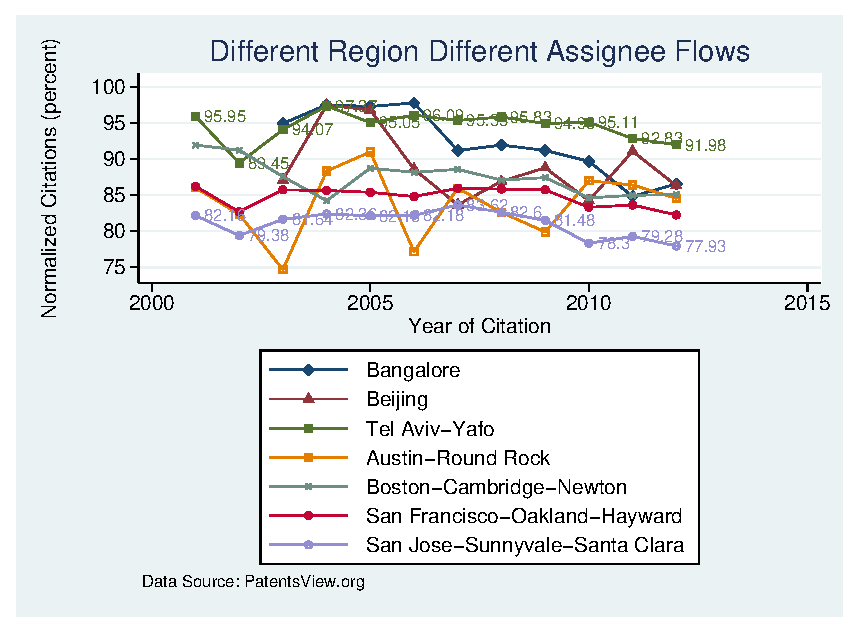
\includegraphics[width=\textwidth]{DiffRegionDiffAssigneeFlows}
  \caption{Non-local and External Flows by Region}
  \label{fig:DiffRegionDiffAssigneeFlows}
\end{centering}
\end{figure}

The rest of this article is organized as follows. In the following section, I present the motivation for empirically designing this study from a selected sampling study. The section following that proposes the hypotheses I intend to test empirically. The approach I take is to assume prior scholarly results about spillovers as a given, and nuance new insights building on top of these giants. The following section on research design presents the constructs created for computing complexity, as well as a discussion on the methodology of the research. My initial, incomplete results are then presented, and a conclusion is drawn of this article as very much a work in progress.

\section{Motivation}
I motivate this study with a small sample analysis of the knowledge spillover characteristics of a selected sample of seven regions across continents, and technological specialization and IPR strength. In each of Figure ~\ref{fig:SameRegionDiffAssigneeFlows}, Figure ~\ref{fig:DiffRegionDiffAssigneeFlows}, Figure ~\ref{fig:SameRegionSameAssigneeFlows} and Figure ~\ref{fig:DiffRegionSameAssigneeFlows}, citation counts of regions are expressed as a normalized percentage number (so as to be able to fairly compare across regions with vastly different pools of knowledge and inventors). Figure ~\ref{fig:SameRegionDiffAssigneeFlows}  already demonstrated that the northern California regions stood out in terms of the extent of local knowledge spillovers to other firms. Scholars have explained this using the mechanism of employee mobility \citep{Almeida1999}. Figure ~\ref{fig:DiffRegionDiffAssigneeFlows}, on the other hand demonstrates that Tel Aviv-Yafo in Israel stands out as accounting of the highest proportion of flows to external firms in external locations. The employee mobility explanation may not be able explain the phenomenon here. Figure ~\ref{fig:SameRegionSameAssigneeFlows} suggests that the Bangalore region sees very little local knowlege spillovers at all, while Figure ~\ref{fig:DiffRegionSameAssigneeFlows} suggests that the Bangalore region flows are dominated by those to the multinational parent location. These disparate spillover behaviors across locations have been attempted to be explained by scholars (e.g., \cite{Zhao2006, Singh2007}) by slicing the problem in a specific context (e.g., of an MNC Parent - MNC Subsidiary). This rather wide disparity between a selection of inventing locations, provides us with the context to dive into the understanding the mechanisms that underlie this divergence in knowledge spillover patters across regions in the aggregate without making simplifying assumptions.

\begin{figure}[h]
\begin{centering}
  \includegraphics[width=\textwidth]{SameRegionSameAssigneeFlows}
  \caption{Local and Internal Flows by Region}
  \label{fig:SameRegionSameAssigneeFlows}
\end{centering}
\end{figure}


\begin{figure}[h]
\begin{centering}
  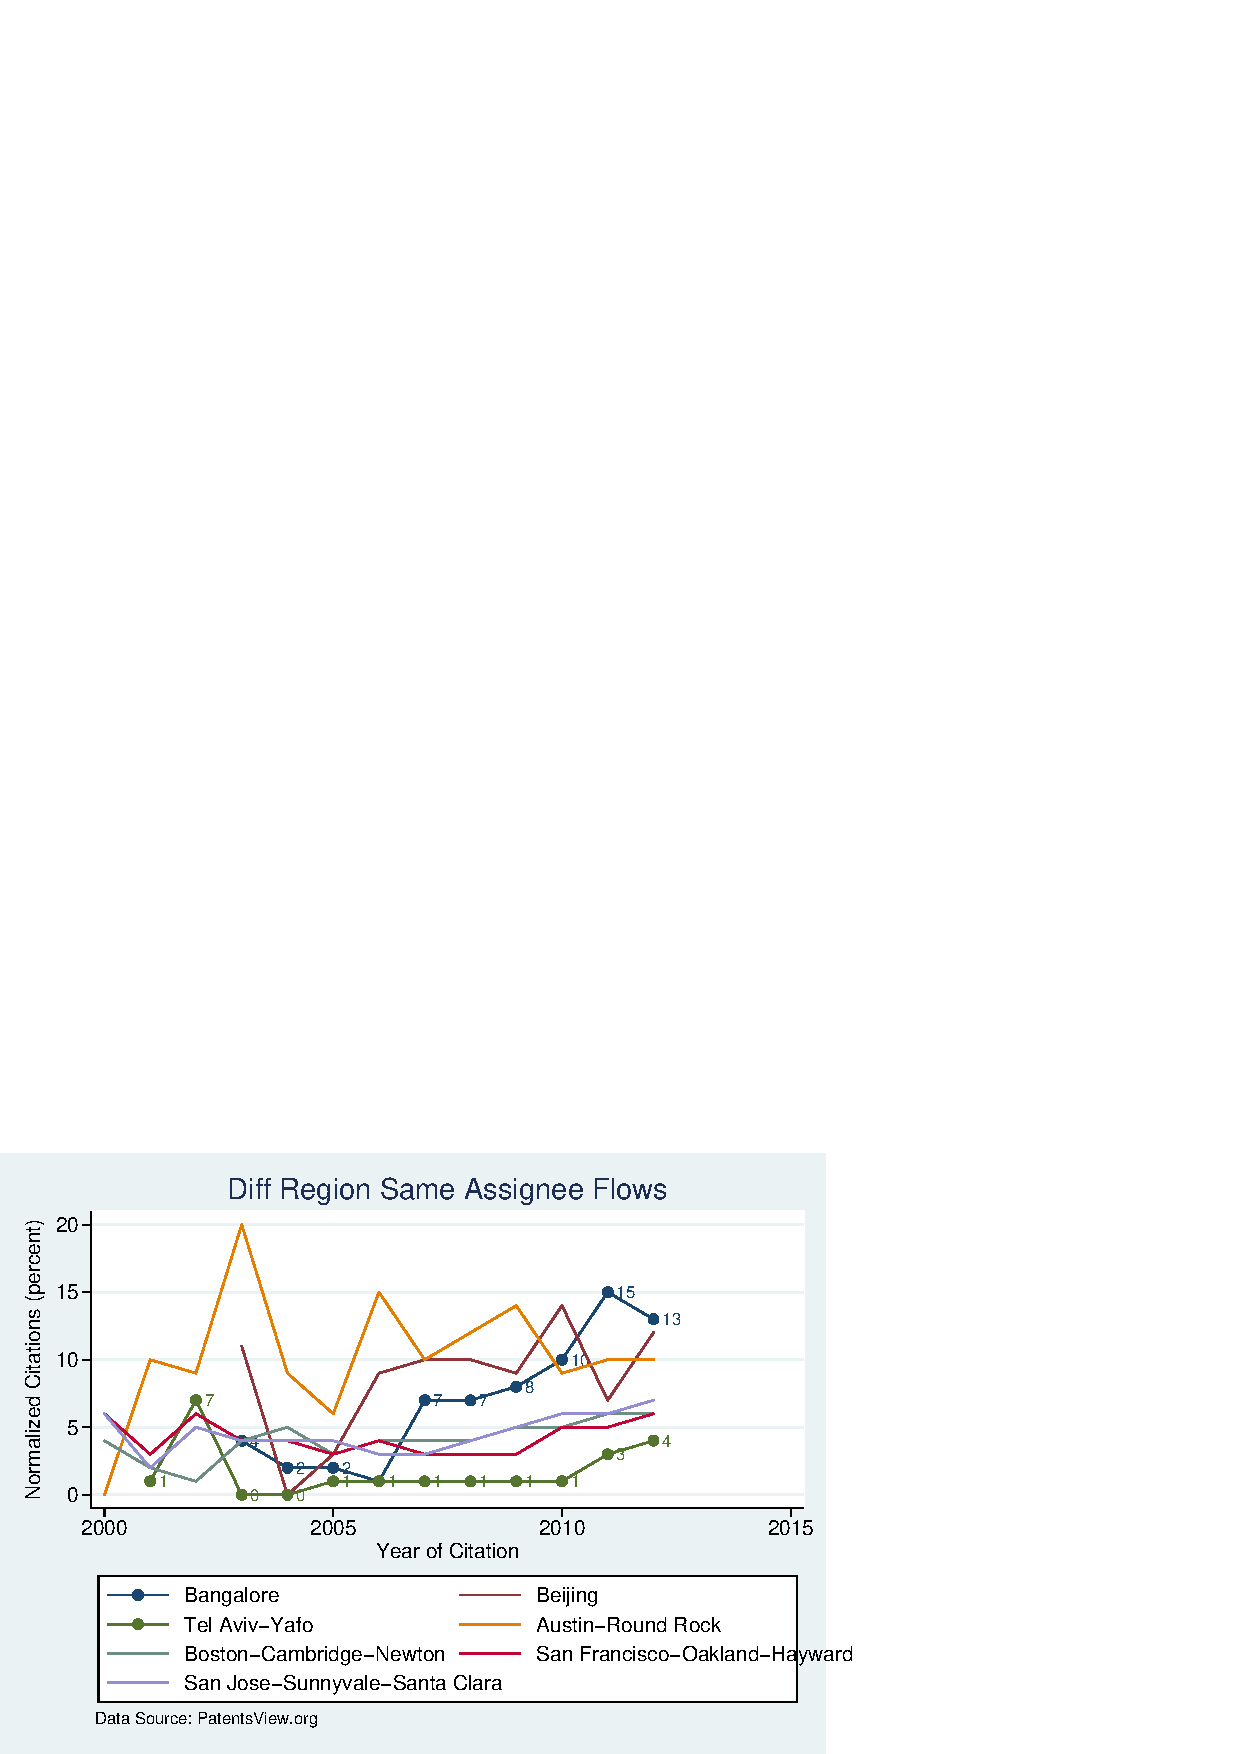
\includegraphics[width=\textwidth]{DiffRegionSameAssigneeFlows}
  \caption{Non-local and Internal Flows by Region}
  \label{fig:DiffRegionSameAssigneeFlows}
\end{centering}
\end{figure}


\section{Theory}
Our approach toward theory building is assume the premise presented by prior scholars as valid to start, and then proceed step by step to nuance those arguments based on our arguments about the interplay of path dependence of the priors of the region, the level of complexity of the inventions produced and the relative strength of the intellectual property rights environment.  Building off on \cite{Jaffe1993}, I propose hypothesis 1 consistent with the priors supported in northern California.

\begin{hypothesis}{\\Hypothesis 1: The higher the number of local citations made by inventors from a region, the higher the number of overall citations received by inventors from that region}\end{hypothesis}

I then build on top of \cite{Zhao2006} and \cite{Singh2007} to propose hypothesis 2.
\begin{hypothesis}{\\Hypothesis 2: The number of overall citations received by inventors from a region is negatively related with the strength of the IPR environment of the region}\end{hypothesis}

Scholars \citep{Yayavaram2008, Baldwin2015}, have argued that increased interaction with a larger number of components creates organizational impediments to an increase in reusability of prior work. In the presence of a stronger differential in the IPR environments between inventing locations, \cite{Zhao2006} suggests that organizational mechanisms may stand to counter the treat posed by weaker property rights. In a similar vein, I argue that a differential in the IPR rights environment creates the organizational response to increase complexity of the inventions shared across country and IPR boundaries. 

\begin{hypothesis}{\\Hypothesis 3: The number of overall citations received by inventors from a region is positively related with the complexity of the invention}\end{hypothesis}

Finally, departing from prior scholarship, I suggest that path dependence would require that the inventing characteristics of locations are deeply embedded in their past. This would therefore suggest that past knowledge flow patters should strongly predict future knowledge flow patters.

\begin{hypothesis}{\\Hypothesis 4a: The number of overall citations received by inventors from a region in a particular period is positively related to the number of citations received by inventors from that region in prior period}\end{hypothesis}

Hypothesis 4b is the logical conclusion from applying hypotheses 3 and 4a, suggesting therefore that the requirements of developing inventions of high complexity may lead firms to strengthen the prior attributes of the patenting region.

\begin{hypothesis}{\\Hypothesis 4b: The effect of Hypothesis 4a is stronger for inventions of high complexity}\end{hypothesis}

\section{Research Design}
\subsection{Complexity}
I construct my measure of complexity based interactions between the different patent sub-classes. Since each of the interactions between patent sub-classes may introduce a new interaction, I model interactions on a binomial function. Specifically, when \verb|subclass| represents the number of distinct patent sub-classes, I define  \verb|interaction(subclass)| as follows:

\begin{displaymath}
   interaction(subclass) = \left\{
     \begin{array}{lr}
       1 & : subclass \leq 2 \\
       \binom{subclass}{2} & : subclass > 2 \\
     \end{array}
   \right.
\end{displaymath} 

I would expect, from a user perspective that the more number of contexts in which the patent is valuable, the lower should be the complexity. If \verb|complexity| represents my measure of the complexity of the patent, and \verb|usage contexts| represents the number of distinct contexts where the patent is found valuable, I should expect the following relationship to hold:
\begin{center}$ \verb|Complexity| \propto \frac{1}{usage \ contexts} $ \end{center}
Similarly, from an inventor perspective, the more the number of contexts that the patent is built on, the higher should be the complexity. A patent that is developed without citing any other patents is an extreme case of lowest complexity, while one that requires to be built upon several \verb|source contexts| is properly understood as being more complex. 

The relationship between \verb|source contexts| and \verb|complexity| is therefore a normal one as depicted below.
\begin{center}$ \verb|complexity| \propto source \ contexts $ \end{center} 

Using the principles above, I therefore develop the following definition of complexity.
\begin{center}$ \verb|complexity| = \frac{interaction(subclass_{\text{cited}})}{interaction(subclass_{\text{patent}})} $ \end{center}

By the definition above, a patent that cites no patents (and hence has $subclass_{\text{cited}} = 0$) but is itself assigned to 4 sub-classes (and hence has $subclass_{\text{patent}} = 4$) will have a raw Complexity score of $\frac{1}{\binom{4}{2}} = 0.16$. If the patent itself had been assigned onto to 2 sub-classes, the raw complexity score would have been just 1. Therefore, the more the number of patent sub-classes a patent is assigned to, the lower its complexity score (by a square term). A similar but inverse relationship would hold for sub-classes arising out of cited patents. Here, I take a set union of patent sub-classes assigned to each cited patent, and use that count to determine the value of the \verb|interaction| function.

\subsection{IPR Classification}
A review of the academic literature surrounding the construction of IPR indexes indicated that there were several, as was also evident in \cite{Zhao2006} constructing a composite measure for the purposes of her article. \cite{Lesser2010} provides an alternative, composite scoring system that includes the following components: protectable subject matter, membership in convention, enforcement, administration and duration of protection. I have therefore used the scores generated by \cite{Lesser2010} for the purposes of this study. The extensive table of IPR scores has not been presented here to adhere to the page restriction, but can be made available on request. The listing has several countries for which scores have not been provided. However none of the top patenting nations were among them, and I therefore chose to go along with this scale.% presented in Table ~\ref{long}

\subsection{Data Source}
I derive all patents data for this study from patentsview.org. The dataset considered is for all USPTO patents filed in the period 1976 to 2015. For the IPR Scores, I rely on the scores generated by \cite{Lesser2010}. For country definitions, I use the resources provided by \href{http://thematicmapping.org/downloads/world_borders.php}{Thematic Mapping}. To determine if spillovers are local, I use a composite data source as described in the following. For locations in the United States, it has been standard to use Metropolitan Statistical Areas (MSA) for analyses related to economic geography. Such standardized data is unavailable for non-US locations. Urban areas are a close substitute for  economic centers, and I therefore determine to use one such definition for non-US locations. My data source for MSA of US locations is \href{http://www.census.gov/geo/maps-data/data/cbf/cbf_msa.html}{the US census} and that for urban areas for world wide locations is \href{http://www.naturalearthdata.com/downloads/10m-cultural-vectors/}{Natural Earth Data}.
 
This automatically raises conflicting definitions for locations in the United States. So that the MSA definitions take precedence, I eliminated all data pertaining to US locations from the Natural Earth urban centers data and integrated this with the MSA information. With this I  generated a single database of location information for economic centers around the world. A sample region definition is depicted in Figure ~\ref{fig:SanJose}. Here all points in the yellow region are considered to fall within the San Jose-Sunnyvale-Santa Clara, CA MSA. In Figure ~\ref{fig:Bangalore}, I present a non-MSA example of a geographic definition based on the urban centers data from \href{http://www.naturalearthdata.com/downloads/10m-cultural-vectors/}{Natural Earth Data}. As will be noticed in Figure ~\ref{fig:Bangalore}, the Bangalore urban center is seen to include parts of Hosur as well.

\subsection{Unit of Analysis}
The unit of analysis for this study is the \verb|region| - \verb|year|

\subsection{Dependent Variable}
My primary dependent variable is the number of citations received by a region in a year. Being a count variable, I use a negative binomial estimation method (xtnbreg in \Stata)\\\\

\subsection{Explanatory Variables}
\subsubsection{Citations Made}
My primary explanatory variables are the four counts of Citations Made along the two dimensions of same/different region and same/different assignee
While most patents have multiple inventors, and some patents also have multiple assignees, my question requires us to associate a single location to the inventor of a patent, and a single location for the assignee of the patent. For the inventor location, I tabulate the count of each of the regions that each inventor is a resident of at the time of the filing of the patent application. In doing so, I treat all inventors equally and allocate the most frequently occurring location as the location of the inventor for that patent. In case of a tie, I assign the location of the first inventor (given by the sequence number of the inventor on the patent) as the location of the inventor of the patent. 
\\\\
For the assignee location, I treat multiple assignees as having been granted separate patents. I do this since the number of patents with multiple assignees is small, and so as to not lose potentially valuable information.



\begin{table}
\begin{center}
\begin{spacing}{0.9}
{
\def\sym#1{\ifmmode^{#1}\else\(^{#1}\)\fi}
\begin{longtable}{l*{2}{c}}
\caption{Effect of Geographic Distribution of Citations Made on Citations Received \label{eflowsreg}}\\
\hline\hline\endfirsthead\hline\endhead\hline\endfoot\endlastfoot
                    &\multicolumn{1}{c}{(1)}&\multicolumn{1}{c}{(2)}\\
                    &\multicolumn{1}{c}{Citations Received}&\multicolumn{1}{c}{Citations Received}\\
\hline
Citations Received  &                     &                     \\
Citations Made to [Same Region, Same Assignee]&   0.0000304\sym{***}&    0.000213         \\
                    &      (5.56)         &      (0.00)         \\
[1em]
Citations Made to [Same Region, Different Assignee]&  0.00000743\sym{*}  &   0.0000599         \\
                    &      (2.37)         &      (0.00)         \\
[1em]
Citations Made to [Different Region, Same Assignee]&-0.000000348         &  0.00000249         \\
                    &     (-0.09)         &      (0.00)         \\
[1em]
Citations Made to [Different Region, Different Assignee]& -0.00000296\sym{***}&   0.0000135         \\
                    &     (-5.55)         &      (0.00)         \\
[1em]
Citations Made to [Other]& -0.00000169         &   0.0000469         \\
                    &     (-1.54)         &      (0.01)         \\
[1em]
Log (Num Patents)   &      0.0132         &      -0.462         \\
                    &      (0.60)         &     (-0.00)         \\
[1em]
Log (Patent Pool Size)&       0.642\sym{***}&       2.382         \\
                    &     (19.36)         &      (0.01)         \\
[1em]
Constant            &      -5.636\sym{***}&      -41.82         \\
                    &    (-23.45)         &         (.)         \\
\hline
ln\_r                &                     &                     \\
Constant            &       0.390\sym{**} &                     \\
                    &      (3.07)         &                     \\
\hline
ln\_s                &                     &                     \\
Constant            &       4.448\sym{***}&                     \\
                    &     (25.14)         &                     \\
[1em]
Year Dummy          &         Yes         &         Yes         \\
[1em]
Region Fixed Effects &          No         &         Yes         \\
\hline
Observations        &        2624         &        2624         \\
\hline\hline
\multicolumn{3}{l}{\footnotesize \textit{t} statistics in parentheses}\\
\multicolumn{3}{l}{\footnotesize \sym{*} \(p<0.05\), \sym{**} \(p<0.01\), \sym{***} \(p<0.001\)}\\
\end{longtable}
}

\end{spacing}
\end{center}
\end{table}

\subsection{Control Variables}
\subsubsection{Size of the patent pool, and Number of patents generated in a region - year}
Since the priors of the region may themselves explain the extent of citations received, I control for both the number of patents generated that year, as well as the aggregate pool of patents invented within that region. The reason both variables are logged is because of the exponential nature of the estimation method used.


\section{Results}
\subsection{Spillover Effects}
Table ~\ref{eflowsreg} presents the preliminary results from my negative binomial regression. The first model uses year dummies but does not include region fixed effects, while the second includes both. As evident, the effects do not seem stable and much empirical work will be needed to determine the right identification method. A couple of approaches that are planned to be tried are to look at controlling for technology class, as regions may vary widely on this aspect. As indicated at the outset, the empirical aspect of this article remains work in progress.

\section{Limitations and Looking Ahead}
I started this study attempting to understand if I could bring three mechanisms to bear together in explaining the heterogeneity in knowledge flows across regions. While there seems to be theoretical promise to exploring this question, this was a study too big to have been completed within the constraints of a term. Specifically, the endeavor has exposed me to the challenges to demonstrating empirically driven work with the objective of building theory. I intend to continue to pursue this further and integrate the IPR level data and complexity data to the flows. In addition, I plan to explore the prospect of controlling for technology classes, and see if that may lead to a strong result.  

\section{Acknowledgements}
I am greatly indebted to Pranav Garg for having emphasized the importance of picking up skills in using Stata while still in the first year. While I might have not done as much justice to it, I cannot imagine having make as much empirical progress on this project if not for that early start. I am also indebted to him for having pushed me to see the theoretical relevance and contribution of empirical work.

I am also grateful to Sai Yayavaram for having introduced me to the literature on innovation, and for having hand held me with working on the patents data. Indeed many of the ideas underlying this article owe their origin to him. All mistakes though, remain entirely mine.

\singlespacing
\bibliography{/Users/aiyenggar/OneDrive/code/bibliography/ae,/Users/aiyenggar/OneDrive/code/bibliography/fj,/Users/aiyenggar/OneDrive/code/bibliography/ko,/Users/aiyenggar/OneDrive/code/bibliography/pt,/Users/aiyenggar/OneDrive/code/bibliography/uz} 
\bibliographystyle{apalike}


\appendix
\begin{figure}[h]
\begin{centering}
  \includegraphics[width=\textwidth]{SanJose}
  \caption{Geographic Definition of San Jose-Sunnyvale-Santa Clara, CA}
   \label{fig:SanJose}
\end{centering}
\end{figure}


\begin{figure}[h]
\begin{centering}
  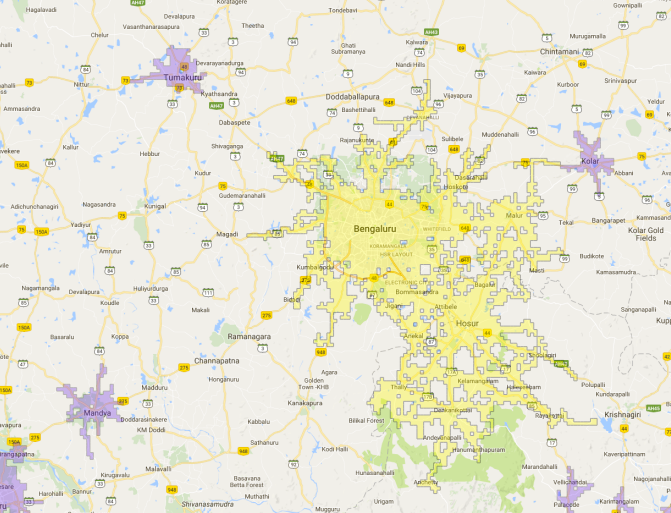
\includegraphics[width=\textwidth]{Bangalore}
  \caption{Geographic Definition of Bangalore}
   \label{fig:Bangalore}
\end{centering}
\end{figure}



\end{document}

\begin{comment}

\cite{Zhao2006} argues that competing firms may have a lower ability to imitate when the value of technology is highly dependent on the proprietary firm\textquotesingle s internal resources. We contend that that assumption is weakened significantly if the knowledge of this technology is codified and published, and when published work on related technologies cite a common prior art. \cite{Zhao2006} herself cites \cite{Kogut1993} suggesting that difficult to codify knowledge lends itself to more efficient transfer within the firm. Drawing on \cite{Cohen2000}, we thereby conclude that firms would have a greater incentive to keep such highly dependent technology developed in weaker IPR countries secret, rather than make this knowledge public. While \cite{Zhao2006} highlights the strength of internal firm linkages in identifying and appropriating the knowledge generated in weak IPR location subsidiaries, she does not emphasize the importance of secrecy. Indeed, she uses patenting data from weaker IPR location offices to substantiate her hypothesis, which we believe actually weakens her argument for the strength of internal firm linkages.

\begin{longtable}{|p{0.5\textwidth}|p{0.30\textwidth}|}
\caption{Countries and their IPR scores \citep{Lesser2010}\label{long}}\\
 
 \hline\textbf{Country}&\textbf{IPR Score}\\\hline
 \endfirsthead
 
 \hline\textbf{Country}&\textbf{IPR Score}\\\hline
 \endhead
 
 \hline
 \endfoot
 
 \hline
 \endlastfoot
Afghanistan& \\\hline
Albania&4.7682 \\\hline
Algeria&2.7608 \\\hline
Angola&1.8734 \\\hline
Anguilla& \\\hline
Antigua and Barbuda& \\\hline
Argentina&5.4684 \\\hline
Armenia&4.4032 \\\hline
Aruba& \\\hline
Australia&11.1872 \\\hline
Austria&9.4024 \\\hline
Azerbaijan&3.1358 \\\hline
Bahamas& \\\hline
Bahrain&5.7736 \\\hline
Bangladesh&2.3664 \\\hline
Barbados& \\\hline
Belarus&3.2344 \\\hline
Belgium&9.6096 \\\hline
Belize& \\\hline
Benin& \\\hline
Bermuda& \\\hline
Bhutan&4.9300 \\\hline
Bolivia&4.2752 \\\hline
Bosnia and Herzegovina&2.9580 \\\hline
Botswana&6.2666 \\\hline
Brazil&5.2612 \\\hline
British Virgin Islands& \\\hline
Brunei Darussalam&5.4230 \\\hline
Bulgaria&5.3598 \\\hline
Burkina Faso&3.5496 \\\hline
Burma& \\\hline
Cambodia&1.9720 \\\hline
Cameroon&2.1692 \\\hline
Canada&11.1872 \\\hline
Cayman Islands& \\\hline
Central African Republic&1.9720 \\\hline
Chad&1.5776 \\\hline
Chile&9.2152 \\\hline
China&6.1586 \\\hline
Colombia&6.2572 \\\hline
Congo&1.8734 \\\hline
Cook Islands& \\\hline
Costa Rica&6.8388 \\\hline
Cote d'Ivoire&2.0706 \\\hline
Croatia&5.8528 \\\hline
Cuba& \\\hline
Cyprus&7.2526 \\\hline
Czech Republic&6.4444 \\\hline
Democratic Republic of the Congo&3.8260 \\\hline
Denmark&11.7788 \\\hline
Djibouti& \\\hline
Dominica& \\\hline
Dominican Republic& \\\hline
Ecuador&3.7822 \\\hline
Egypt&2.7608 \\\hline
El Salvador&3.3524 \\\hline
Equatorial Guinea& \\\hline
Estonia&9.1166 \\\hline
Ethiopia&2.6622 \\\hline
Fiji& \\\hline
Finland&11.3844 \\\hline
France&10.3984 \\\hline
French Guiana&10.3984 \\\hline
Gabon&2.8594 \\\hline
Gambia&2.8594 \\\hline
Georgia&4.9106 \\\hline
Germany&10.4970 \\\hline
Ghana&4.5904 \\\hline
Greece&5.4878 \\\hline
Greenland& \\\hline
Guadeloupe& \\\hline
Guam& \\\hline
Guatemala&3.3524 \\\hline
Guernsey& \\\hline
Guinea&1.7748 \\\hline
Guinea-Bissau& \\\hline
Guyana&2.5636 \\\hline
Haiti&1.7748 \\\hline
Honduras&3.2100 \\\hline
Hong Kong&8.0852 \\\hline
Hungary&7.6376 \\\hline
Iceland&10.1912 \\\hline
India&4.0974 \\\hline
Indonesia&4.5018 \\\hline
Iran (Islamic Republic of)&1.7748 \\\hline
Iraq&1.4790 \\\hline
Ireland&9.6290 \\\hline
Isle of Man& \\\hline
Israel&8.6236 \\\hline
Italy&6.8488 \\\hline
Jamaica&2.9580 \\\hline
Japan&10.2012 \\\hline
Jersey& \\\hline
Jordan&6.5430 \\\hline
Kazakhstan&2.6622 \\\hline
Kenya&3.7822 \\\hline
Korea, Democratic Republic of& \\\hline
Korea, Republic of&7.1640 \\\hline
Kuwait&4.0426 \\\hline
Kyrgyzstan&3.4864 \\\hline
Lao People's Democratic Republic&1.9720 \\\hline
Latvia&6.0500 \\\hline
Lebanon&2.4650 \\\hline
Lesotho& \\\hline
Liberia&3.0566 \\\hline
Libyan Arab Jamahiriya& \\\hline
Liechtenstein& \\\hline
Lithuania&7.4404 \\\hline
Luxembourg&8.8302 \\\hline
Macau& \\\hline
Madagascar&2.9580 \\\hline
Malawi&3.2538 \\\hline
Malaysia&5.1820 \\\hline
Mali&2.7608 \\\hline
Malta& \\\hline
Mauritania&2.4650 \\\hline
Mauritius&5.3244 \\\hline
Mexico&4.8668 \\\hline
Monaco& \\\hline
Mongolia&3.4072 \\\hline
Montenegro& \\\hline
Morocco&5.8628 \\\hline
Mozambique&2.4650 \\\hline
Namibia&4.4370 \\\hline
Nepal&2.2678 \\\hline
Netherlands Antilles&11.3844 \\\hline
Netherlands&11.3844 \\\hline
New Caledonia& \\\hline
New Zealand&11.8774 \\\hline
Nicaragua&5.0740 \\\hline
Niger&2.8594 \\\hline
Nigeria&3.2100 \\\hline
Northern Mariana Islands& \\\hline
Norway&10.1912 \\\hline
Oman&7.0360 \\\hline
Pakistan&4.1074 \\\hline
Palau& \\\hline
Palestine& \\\hline
Panama&5.2164 \\\hline
Papua New Guinea&2.0706 \\\hline
Paraguay&3.6836 \\\hline
Peru&5.3892 \\\hline
Philippines&4.1074 \\\hline
Poland&7.5390 \\\hline
Portugal&8.3278 \\\hline
Puerto Rico& \\\hline
Qatar&7.6470 \\\hline
Republic of Moldova&4.1218 \\\hline
Reunion& \\\hline
Romania&6.3558 \\\hline
Russia&4.0332 \\\hline
Saint Barthelemy& \\\hline
Saint Kitts and Nevis& \\\hline
Saint Lucia& \\\hline
Saint Pierre and Miquelon& \\\hline
San Marino& \\\hline
Saudi Arabia&4.2398 \\\hline
Senegal&2.9580 \\\hline
Serbia&4.4470 \\\hline
Seychelles& \\\hline
Sierra Leone&2.1692 \\\hline
Singapore&11.6802 \\\hline
Slovakia&7.0460 \\\hline
Slovenia&8.3716 \\\hline
Solomon Islands& \\\hline
South Africa&7.2432 \\\hline
Spain&8.6236 \\\hline
Sri Lanka&3.0566 \\\hline
Sudan&1.4790 \\\hline
Suriname&3.6482 \\\hline
Svalbard& \\\hline
Swaziland&4.2946 \\\hline
Sweden&11.6802 \\\hline
Switzerland&11.4830 \\\hline
Syrian Arab Republic&3.5596 \\\hline
Taiwan&7.2626 \\\hline
Tajikistan&1.9720 \\\hline
Thailand&4.0974 \\\hline
The former Yugoslav Republic of Macedonia& \\\hline
Togo&2.7608 \\\hline
Trinidad and Tobago&5.1626 \\\hline
Tunisia&5.8528 \\\hline
Turkey&6.9474 \\\hline
Turkmenistan& \\\hline
Turks and Caicos Islands& \\\hline
Uganda&2.4650 \\\hline
Ukraine&3.7822 \\\hline
United Arab Emirates&6.4090 \\\hline
United Kingdom&10.2012 \\\hline
United Republic of Tanzania&2.5636 \\\hline
United States Virgin Islands&10.0040 \\\hline
United States&10.0040 \\\hline
Uruguay&8.2192 \\\hline
Uzbekistan&3.6388 \\\hline
Venezuela&3.6144 \\\hline
Vietnam&4.2752 \\\hline
Yemen&2.0706 \\\hline
Zambia&2.9580 \\\hline
Zimbabwe&2.9142 \\\hline
\end{longtable}



\end{comment}
